\section{产品状态：从前代商业化到新代实物}

Atlas 950 的产业意义在于，华为正在把超节点的 scale-up 域从 384 卡扩展到多机柜的千卡乃至 8,192 卡设计。其目标不是简单堆叠芯片，而是通过 UnifiedBus 2.0、统一地址空间、集合通信、容错和编译运行时协同，把多个计算柜与互联柜组织为单逻辑机。若这一架构成立，系统瓶颈会从单卡峰值转向互联带宽与时延、HBM/池化内存、供电、液冷、机柜集成、故障恢复和软件利用率。

\begin{figure}[htbp]
\centering
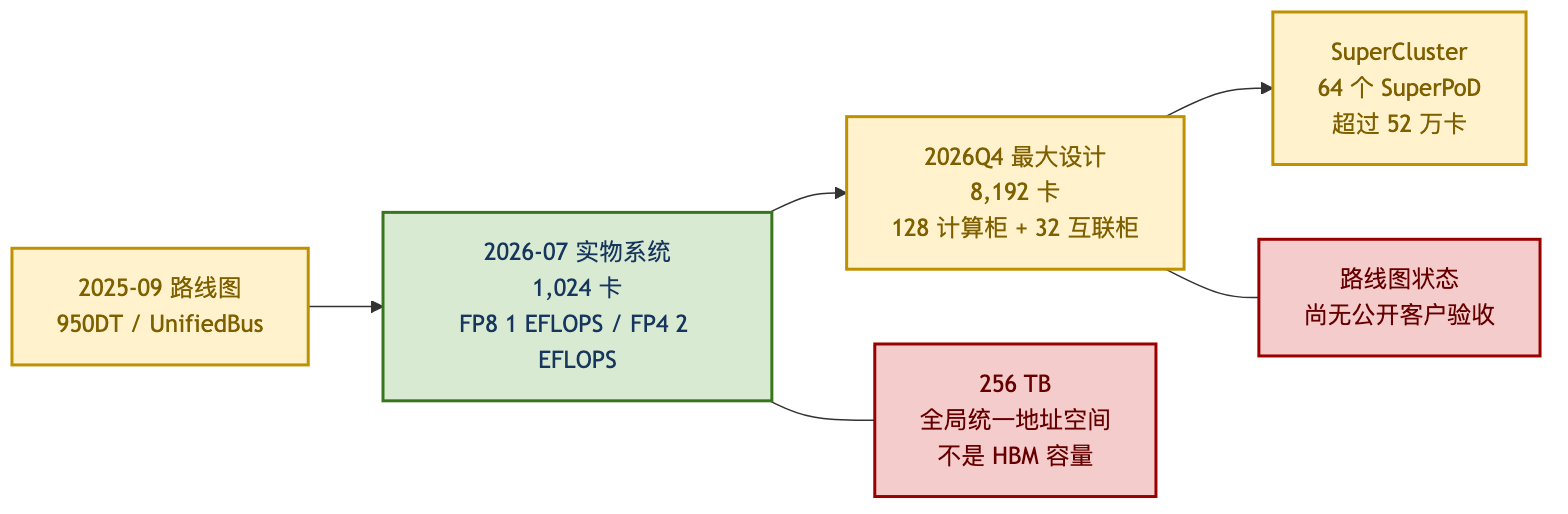
\includegraphics[width=\textwidth]{exhibits/architecture_state.png}
\caption{Atlas 950 从路线图到实物、最大设计与集群边界}
\sourcenote{基于华为 H1--H4 官方资料绘制；绿色为已公开实物，黄色为路线图，红色为必须保留的定义/状态边界。}
\end{figure}

图中最重要的不是卡数递增，而是证据状态递进：1,024 卡系统已经展示；8,192 卡是最大设计与 2026Q4 可用计划；SuperCluster 又是 64 个 SuperPoD 的 scale-out 层。256TB 只描述全局统一地址空间，不能替代 950DT 单卡 144GB HiZQ 2.0 的存储规格。

\begin{exhibitbox}[华为超节点产品状态表]
\begin{tabularx}{\textwidth}{L{2.8cm}L{2.8cm}L{2.5cm}X}
\toprule
\textbf{产品/边界} & \textbf{公开规模} & \textbf{截至截止日状态} & \textbf{正确解读}\\
\midrule
Atlas 900 A3 / CloudMatrix384 & 384 卡 & 前代商业部署 & 证明华为有前代产品化经验，不证明 950 供应链\\
昇腾 950DT & 144GB HiZQ 2.0 HBM/卡 & 2026Q4 路线图 & 芯片规格和时间表为前瞻陈述\\
Atlas 950 实物系统 & 1,024 卡 & 2026-07-17 首次公开展示 & 验证实物与系统级指标；未披露客户、站点、功耗、BOM\\
Atlas 950 最大设计 & 8,192 卡、160 柜 & 计划 2026Q4 可用 & 设计上限，不是已经交付或验收\\
Atlas 950 SuperCluster & 64 个 SuperPoD、逾 52 万卡 & 2026Q4 路线图 & scale-out 集群，不是单台 SuperPoD\\
\bottomrule
\end{tabularx}
\sourcenote{华为 2025-09-18、2026-03-02、2026-07-17 官方资料 [H1][H3][H4]。}
\end{exhibitbox}

\section{竞争架构：更大 scale-up 域是一场系统工程押注}

华为 Atlas 950、NVIDIA GB300/Vera Rubin 和 AMD Helios 并非统一口径的“卡数比赛”。NVIDIA 以 CUDA、NVLink/NVSwitch、网络和 OEM 生态构成生产系统护城河；AMD 以 UALink/UEC、开放参考设计和 OEM 灵活性切入；华为则在受限半导体条件下，以更大多机柜 scale-up 域、统一编址和国内软硬件栈提高系统级算力。其优势是主权可控与系统协同，风险是 8,192 卡规模下的良率、故障率、通信效率、软件利用率和运维复杂度。

\begin{exhibitbox}[三种 scale-up 路线比较]
\begin{tabularx}{\textwidth}{L{2.5cm}L{3cm}L{3.2cm}X}
\toprule
\textbf{平台} & \textbf{厂商描述的 scale-up 域} & \textbf{主要护城河} & \textbf{不可直接比较项}\\
\midrule
华为 Atlas 950 & 1,024 卡实物；8,192 卡设计 & UnifiedBus、统一地址空间、国产栈 & 功耗、精度/稀疏口径、独立负载利用率未披露\\
NVIDIA GB300 NVL72 & 72 GPU 机架级 NVLink 域 & CUDA、NVLink/NVSwitch、网络/OEM 生态 & 卡数小不等于系统算力低；性能口径不同\\
AMD Helios & 72 MI455X 开放机架参考设计 & UALink/UEC、开放 OEM/ODM 生态 & 2026 下半年量产部署仍属厂商预期\\
NVIDIA Vera Rubin POD & 5 个专用机柜围绕 NVL72 系统 & 下一代 NVLink、Spectrum-X、BlueField & 当前官方边界并非旧对比材料中的 NVL144\\
\bottomrule
\end{tabularx}
\sourcenote{华为官方 [H1][H3][H4]；NVIDIA、AMD 官方产品资料 [C1][C2][C21]。峰值数字未做跨厂商归一化。}
\end{exhibitbox}

\section{价值池为何向互联、供电和液冷迁移}

当系统从单机或单柜扩展到 160 柜，计算芯片仍是最大价值密度环节，但部署成败越来越由跨柜互联、供配电、热管理和软件调度共同决定。全光 UB-Mesh 带来光引擎、交换、光纤和精密连接的潜在需求，却也可能因 UBoE、CPO/LPO 或 OCS 选择而改变可插拔模块数量。全液冷提高冷板、Manifold、CDU、快接、管路、冷源和监控价值量，但供应商必须经过平台认证、泄漏与长期可靠性验证。大功率系统还需要变压器、UPS/HVDC、母线、配电和备用电源协同，实际价值取决于 MW、拓扑和站点边界。

因此，价值池判断必须使用“数量乘 ASP”之外的第二层约束：产品是否外购、由华为/ODM 内制还是由数据中心业主采购；订单在设备交付还是站点验收后确认；毛利率是否被客户集中度和项目集成稀释；应收与存货是否吞噬利润；技术路线变化是否使单卡价值量下降。没有这些信息，就只能确认工程方向，不能给公司收入。

\section{可计算 TAM 与不可计算 TAM}

合理的公司收入桥应为：客户验收的 SuperPoD 数量 $\times$ 配置结构 $\times$ 每系统该环节数量 $\times$ 合格 ASP $\times$ 上市公司分配份额 $\times$ 交付/验收率。当前官方资料只给出部分配置上限，不给出客户验收数量、系统价格、功耗、端口/模块/CDU/连接器数量、供应商份额和收入节奏。因而本报告不发布货币化 Atlas 950 TAM、A 股 SAM 或公司 SOM。

这并不意味着产业机会为零，而是意味着“可计入估值的公司收入”为零。未来只要客户、数量、BOM 与供应商证据补齐，模型可以从 0 向上更新；当前直接填入一个市场规模会制造无法审计的精确数字。

\begin{keyinsight}[行业判断]
Atlas 950 已把“国产超节点能否做出实物”的问题向前推进一步；尚未回答“8,192 卡能否稳定运行、谁来采购、谁来供货、每个环节赚多少钱”。投资研究的价值正是守住这四个未回答的问题。
\end{keyinsight}
